\documentclass[14pt]{extbook}
\usepackage{multicol, enumerate, enumitem, hyperref, color, soul, setspace, parskip, fancyhdr} %General Packages
\usepackage{amssymb, amsthm, amsmath, latexsym, units, mathtools} %Math Packages
\everymath{\displaystyle} %All math in Display Style
% Packages with additional options
\usepackage[headsep=0.5cm,headheight=12pt, left=1 in,right= 1 in,top= 1 in,bottom= 1 in]{geometry}
\usepackage[usenames,dvipsnames]{xcolor}
\usepackage{dashrule}  % Package to use the command below to create lines between items
\newcommand{\litem}[1]{\item#1\hspace*{-1cm}\rule{\textwidth}{0.4pt}}
\pagestyle{fancy}
\lhead{Makeup Progress Quiz 2}
\chead{}
\rhead{Version ALL}
\lfoot{2790-1423}
\cfoot{}
\rfoot{Summer C 2021}
\begin{document}

\begin{enumerate}
\litem{
Graph the equation below.\[ f(x) = (x-1)^2 + 12 \]\begin{enumerate}[label=\Alph*.]
\begin{multicols}{2}\item 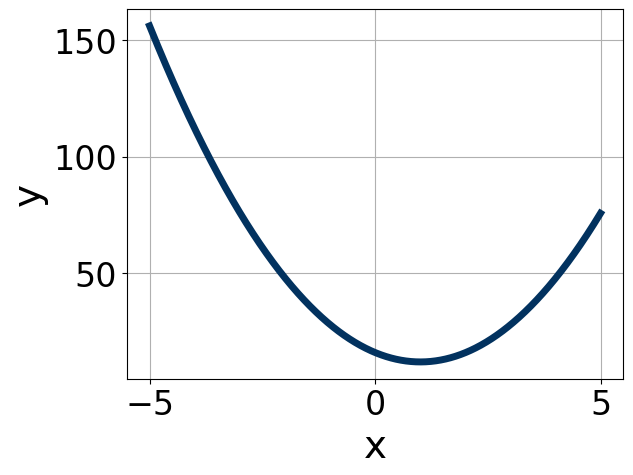
\includegraphics[width = 0.3\textwidth]{../Figures/quadraticEquationToGraphCopyAA.png}\item 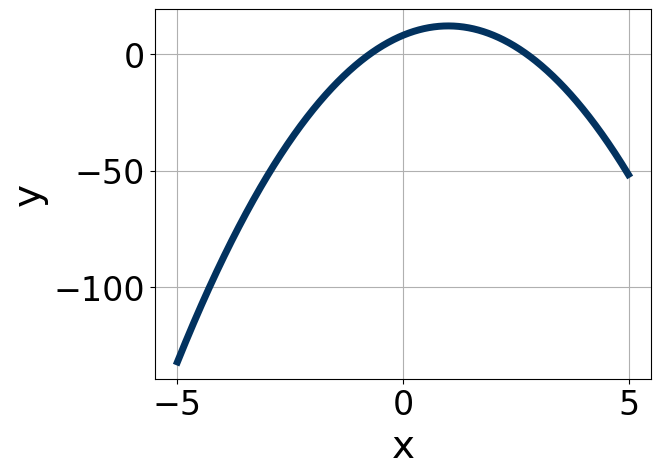
\includegraphics[width = 0.3\textwidth]{../Figures/quadraticEquationToGraphCopyBA.png}\item 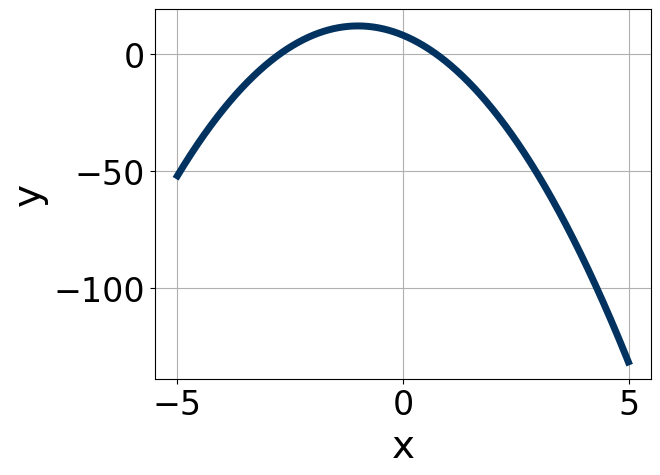
\includegraphics[width = 0.3\textwidth]{../Figures/quadraticEquationToGraphCopyCA.png}\item 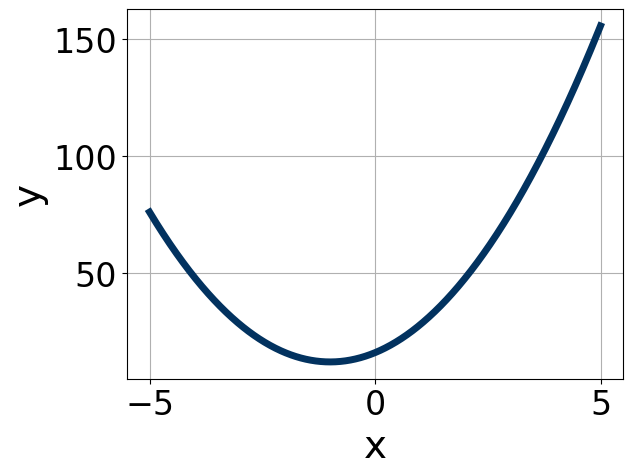
\includegraphics[width = 0.3\textwidth]{../Figures/quadraticEquationToGraphCopyDA.png}\end{multicols}\item None of the above.
\end{enumerate} }
\litem{
Solve the quadratic equation below. Then, choose the intervals that the solutions belong to, with $x_1 \leq x_2$ (if they exist).\[ -12x^{2} -9 x + 2 = 0 \]\begin{enumerate}[label=\Alph*.]
\item \( x_1 \in [-1.22, -0.45] \text{ and } x_2 \in [-0.98, 0.69] \)
\item \( x_1 \in [-14.11, -13.56] \text{ and } x_2 \in [12.66, 13.16] \)
\item \( x_1 \in [-0.3, 0.07] \text{ and } x_2 \in [0.71, 1.12] \)
\item \( x_1 \in [-2.35, -1.93] \text{ and } x_2 \in [10.81, 11.87] \)
\item \( \text{There are no Real solutions.} \)

\end{enumerate} }
\litem{
Factor the quadratic below. Then, choose the intervals that contain the constants in the form $(ax+b)(cx+d); b \leq d.$\[ 16x^{2} -40 x + 25 \]\begin{enumerate}[label=\Alph*.]
\item \( a \in [7.53, 9.57], \hspace*{5mm} b \in [-14, -3], \hspace*{5mm} c \in [1.77, 3.95], \text{ and } \hspace*{5mm} d \in [-8, -4] \)
\item \( a \in [1.91, 3.55], \hspace*{5mm} b \in [-14, -3], \hspace*{5mm} c \in [7.21, 9.2], \text{ and } \hspace*{5mm} d \in [-8, -4] \)
\item \( a \in [3.34, 5.88], \hspace*{5mm} b \in [-14, -3], \hspace*{5mm} c \in [3.86, 4.01], \text{ and } \hspace*{5mm} d \in [-8, -4] \)
\item \( a \in [0.64, 1.35], \hspace*{5mm} b \in [-24, -19], \hspace*{5mm} c \in [0.53, 1.17], \text{ and } \hspace*{5mm} d \in [-23, -16] \)
\item \( \text{None of the above.} \)

\end{enumerate} }
\litem{
Solve the quadratic equation below. Then, choose the intervals that the solutions $x_1$ and $x_2$ belong to, with $x_1 \leq x_2$.\[ 25x^{2} +60 x + 36 = 0 \]\begin{enumerate}[label=\Alph*.]
\item \( x_1 \in [-6.81, -5.76] \text{ and } x_2 \in [-0.36, 0.06] \)
\item \( x_1 \in [-30.51, -28.26] \text{ and } x_2 \in [-30.28, -29.95] \)
\item \( x_1 \in [-3.92, -3.48] \text{ and } x_2 \in [-0.47, -0.38] \)
\item \( x_1 \in [-2.6, -2.14] \text{ and } x_2 \in [-0.95, -0.45] \)
\item \( x_1 \in [-2.12, 0.44] \text{ and } x_2 \in [-1.65, -1.18] \)

\end{enumerate} }
\litem{
Solve the quadratic equation below. Then, choose the intervals that the solutions belong to, with $x_1 \leq x_2$ (if they exist).\[ 19x^{2} +11 x -9 = 0 \]\begin{enumerate}[label=\Alph*.]
\item \( x_1 \in [-20.03, -19.59] \text{ and } x_2 \in [7.1, 8.8] \)
\item \( x_1 \in [-29.09, -27.92] \text{ and } x_2 \in [26.9, 28.8] \)
\item \( x_1 \in [-1.26, -0.72] \text{ and } x_2 \in [-2, 0.9] \)
\item \( x_1 \in [-0.89, -0.22] \text{ and } x_2 \in [0.8, 1.3] \)
\item \( \text{There are no Real solutions.} \)

\end{enumerate} }
\litem{
Graph the equation below.\[ f(x) = (x+3)^2 + 18 \]\begin{enumerate}[label=\Alph*.]
\begin{multicols}{2}\item 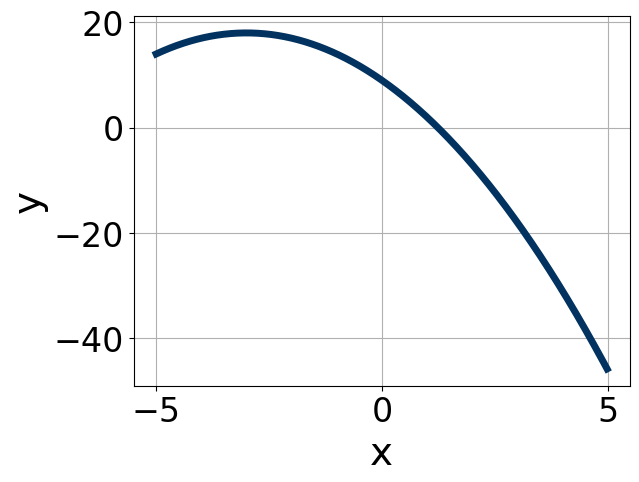
\includegraphics[width = 0.3\textwidth]{../Figures/quadraticEquationToGraphAA.png}\item 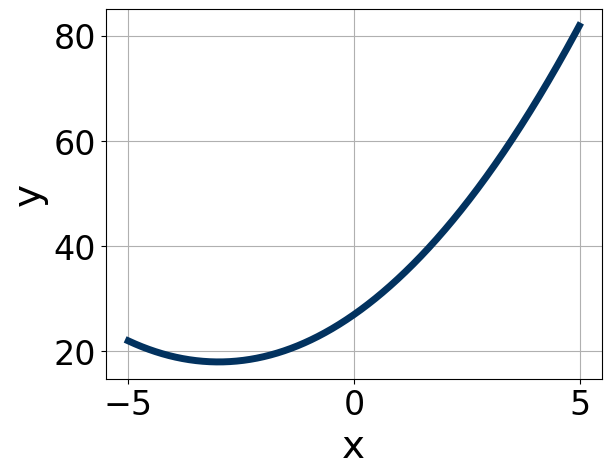
\includegraphics[width = 0.3\textwidth]{../Figures/quadraticEquationToGraphBA.png}\item 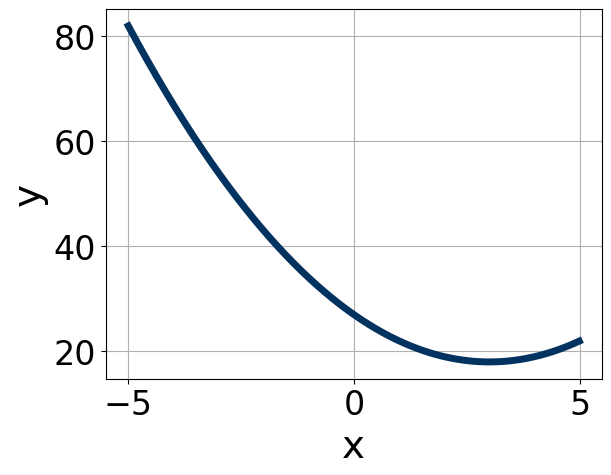
\includegraphics[width = 0.3\textwidth]{../Figures/quadraticEquationToGraphCA.png}\item 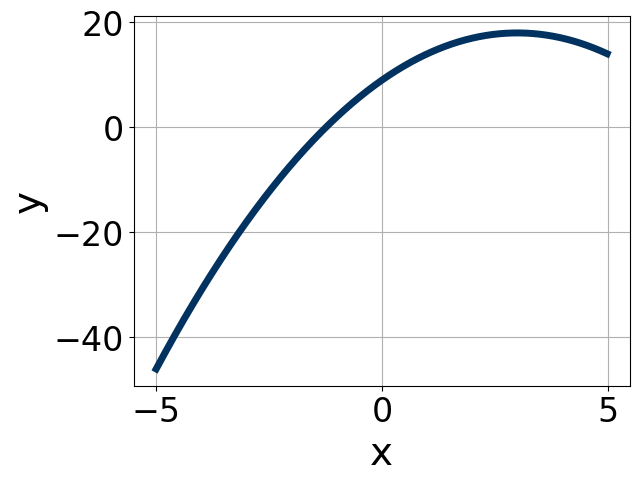
\includegraphics[width = 0.3\textwidth]{../Figures/quadraticEquationToGraphDA.png}\end{multicols}\item None of the above.
\end{enumerate} }
\litem{
Solve the quadratic equation below. Then, choose the intervals that the solutions $x_1$ and $x_2$ belong to, with $x_1 \leq x_2$.\[ 10x^{2} -33 x -54 = 0 \]\begin{enumerate}[label=\Alph*.]
\item \( x_1 \in [-2.15, -1.09] \text{ and } x_2 \in [4.46, 5.37] \)
\item \( x_1 \in [-0.69, -0.37] \text{ and } x_2 \in [12.39, 13.71] \)
\item \( x_1 \in [-2.66, -1.74] \text{ and } x_2 \in [1.04, 3.51] \)
\item \( x_1 \in [-6.77, -5.51] \text{ and } x_2 \in [-1.09, 2.11] \)
\item \( x_1 \in [-12.07, -11.74] \text{ and } x_2 \in [44.34, 46.23] \)

\end{enumerate} }
\litem{
Write the equation of the graph presented below in the form $f(x)=ax^2+bx+c$, assuming  $a=1$ or $a=-1$. Then, choose the intervals that $a, b,$ and $c$ belong to.
\begin{center}
    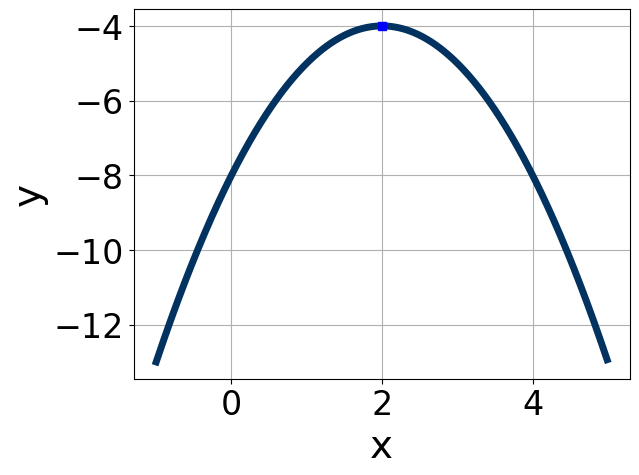
\includegraphics[width=0.5\textwidth]{../Figures/quadraticGraphToEquationA.png}
\end{center}
\begin{enumerate}[label=\Alph*.]
\item \( a \in [1, 2], \hspace*{5mm} b \in [-5, -1], \text{ and } \hspace*{5mm} c \in [-2, 3] \)
\item \( a \in [-3, 0], \hspace*{5mm} b \in [-5, -1], \text{ and } \hspace*{5mm} c \in [-8, -3] \)
\item \( a \in [1, 2], \hspace*{5mm} b \in [3, 6], \text{ and } \hspace*{5mm} c \in [-2, 3] \)
\item \( a \in [-3, 0], \hspace*{5mm} b \in [3, 6], \text{ and } \hspace*{5mm} c \in [-8, -3] \)
\item \( a \in [-3, 0], \hspace*{5mm} b \in [-5, -1], \text{ and } \hspace*{5mm} c \in [-2, 3] \)

\end{enumerate} }
\litem{
Factor the quadratic below. Then, choose the intervals that contain the constants in the form $(ax+b)(cx+d); b \leq d.$\[ 36x^{2} -60 x + 25 \]\begin{enumerate}[label=\Alph*.]
\item \( a \in [3, 5], \hspace*{5mm} b \in [-11, 1], \hspace*{5mm} c \in [11.52, 12.36], \text{ and } \hspace*{5mm} d \in [-9, 1] \)
\item \( a \in [-2, 2], \hspace*{5mm} b \in [-36, -29], \hspace*{5mm} c \in [0.92, 1.31], \text{ and } \hspace*{5mm} d \in [-36, -22] \)
\item \( a \in [9, 19], \hspace*{5mm} b \in [-11, 1], \hspace*{5mm} c \in [2.88, 3.42], \text{ and } \hspace*{5mm} d \in [-9, 1] \)
\item \( a \in [4, 7], \hspace*{5mm} b \in [-11, 1], \hspace*{5mm} c \in [5.85, 6.18], \text{ and } \hspace*{5mm} d \in [-9, 1] \)
\item \( \text{None of the above.} \)

\end{enumerate} }
\litem{
Write the equation of the graph presented below in the form $f(x)=ax^2+bx+c$, assuming  $a=1$ or $a=-1$. Then, choose the intervals that $a, b,$ and $c$ belong to.
\begin{center}
    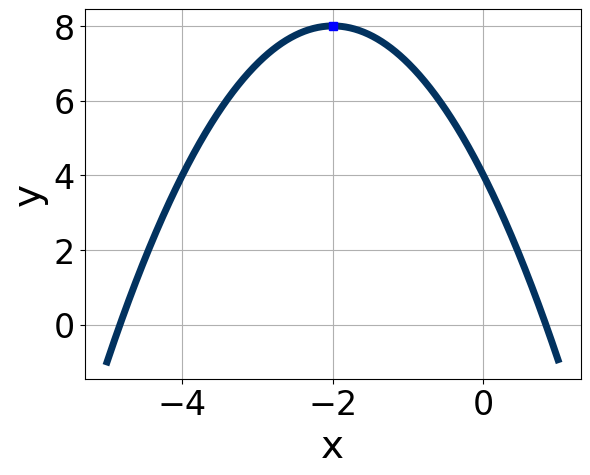
\includegraphics[width=0.5\textwidth]{../Figures/quadraticGraphToEquationCopyA.png}
\end{center}
\begin{enumerate}[label=\Alph*.]
\item \( a \in [1, 2], \hspace*{5mm} b \in [-4, -1], \text{ and } \hspace*{5mm} c \in [10, 15] \)
\item \( a \in [-1, 0], \hspace*{5mm} b \in [-4, -1], \text{ and } \hspace*{5mm} c \in [3, 7] \)
\item \( a \in [1, 2], \hspace*{5mm} b \in [4, 8], \text{ and } \hspace*{5mm} c \in [10, 15] \)
\item \( a \in [-1, 0], \hspace*{5mm} b \in [4, 8], \text{ and } \hspace*{5mm} c \in [3, 7] \)
\item \( a \in [-1, 0], \hspace*{5mm} b \in [4, 8], \text{ and } \hspace*{5mm} c \in [-13, -10] \)

\end{enumerate} }
\litem{
Graph the equation below.\[ f(x) = -(x+4)^2 - 20 \]\begin{enumerate}[label=\Alph*.]
\begin{multicols}{2}\item 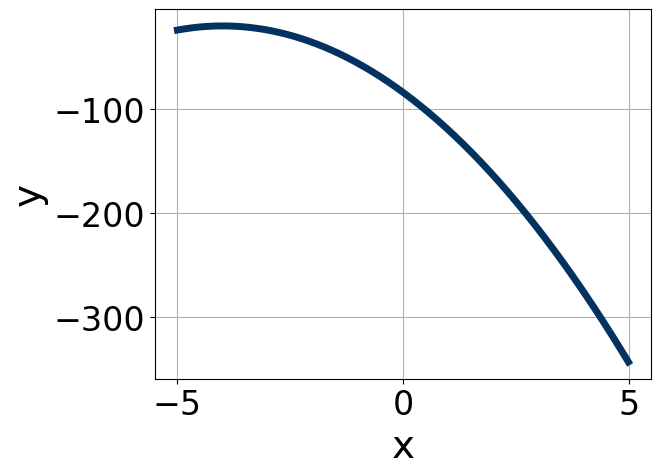
\includegraphics[width = 0.3\textwidth]{../Figures/quadraticEquationToGraphCopyAB.png}\item 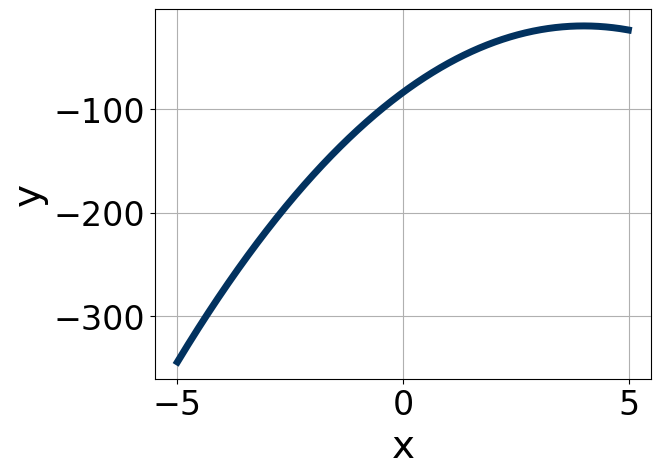
\includegraphics[width = 0.3\textwidth]{../Figures/quadraticEquationToGraphCopyBB.png}\item 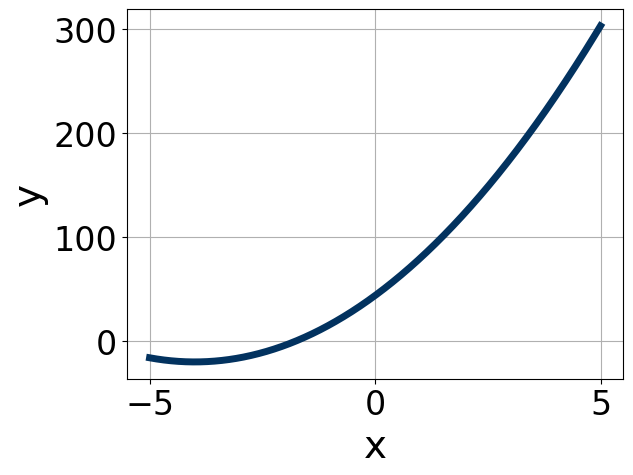
\includegraphics[width = 0.3\textwidth]{../Figures/quadraticEquationToGraphCopyCB.png}\item 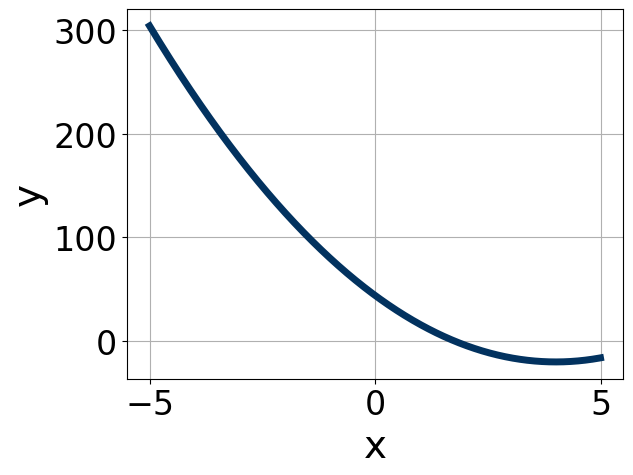
\includegraphics[width = 0.3\textwidth]{../Figures/quadraticEquationToGraphCopyDB.png}\end{multicols}\item None of the above.
\end{enumerate} }
\litem{
Solve the quadratic equation below. Then, choose the intervals that the solutions belong to, with $x_1 \leq x_2$ (if they exist).\[ 14x^{2} +15 x -6 = 0 \]\begin{enumerate}[label=\Alph*.]
\item \( x_1 \in [-1, -0.1] \text{ and } x_2 \in [0.68, 1.66] \)
\item \( x_1 \in [-21, -17.8] \text{ and } x_2 \in [3.87, 5.42] \)
\item \( x_1 \in [-3.1, -0.7] \text{ and } x_2 \in [0.2, 0.53] \)
\item \( x_1 \in [-24.9, -22.7] \text{ and } x_2 \in [22.4, 24.39] \)
\item \( \text{There are no Real solutions.} \)

\end{enumerate} }
\litem{
Factor the quadratic below. Then, choose the intervals that contain the constants in the form $(ax+b)(cx+d); b \leq d.$\[ 36x^{2} -60 x + 25 \]\begin{enumerate}[label=\Alph*.]
\item \( a \in [0.76, 1.62], \hspace*{5mm} b \in [-31, -28], \hspace*{5mm} c \in [0.3, 1.7], \text{ and } \hspace*{5mm} d \in [-32, -28] \)
\item \( a \in [1.55, 2.31], \hspace*{5mm} b \in [-14, -3], \hspace*{5mm} c \in [17.2, 20.8], \text{ and } \hspace*{5mm} d \in [-10, -2] \)
\item \( a \in [4.65, 6.7], \hspace*{5mm} b \in [-14, -3], \hspace*{5mm} c \in [5.4, 8.8], \text{ and } \hspace*{5mm} d \in [-10, -2] \)
\item \( a \in [16.99, 19.36], \hspace*{5mm} b \in [-14, -3], \hspace*{5mm} c \in [1.1, 4.2], \text{ and } \hspace*{5mm} d \in [-10, -2] \)
\item \( \text{None of the above.} \)

\end{enumerate} }
\litem{
Solve the quadratic equation below. Then, choose the intervals that the solutions $x_1$ and $x_2$ belong to, with $x_1 \leq x_2$.\[ 15x^{2} +7 x -36 = 0 \]\begin{enumerate}[label=\Alph*.]
\item \( x_1 \in [-7.9, -2.9] \text{ and } x_2 \in [0.34, 0.74] \)
\item \( x_1 \in [-2.9, -1.3] \text{ and } x_2 \in [0.97, 1.74] \)
\item \( x_1 \in [-10.2, -8.1] \text{ and } x_2 \in [-0.01, 0.28] \)
\item \( x_1 \in [-1, -0.7] \text{ and } x_2 \in [2.3, 3.12] \)
\item \( x_1 \in [-30.5, -24.2] \text{ and } x_2 \in [19.66, 20.07] \)

\end{enumerate} }
\litem{
Solve the quadratic equation below. Then, choose the intervals that the solutions belong to, with $x_1 \leq x_2$ (if they exist).\[ -14x^{2} +7 x + 6 = 0 \]\begin{enumerate}[label=\Alph*.]
\item \( x_1 \in [-0.88, -0.16] \text{ and } x_2 \in [0.78, 1] \)
\item \( x_1 \in [-19.54, -19.21] \text{ and } x_2 \in [19.4, 20.44] \)
\item \( x_1 \in [-0.96, -0.86] \text{ and } x_2 \in [0.33, 0.55] \)
\item \( x_1 \in [-13.63, -13.3] \text{ and } x_2 \in [6, 7.07] \)
\item \( \text{There are no Real solutions.} \)

\end{enumerate} }
\litem{
Graph the equation below.\[ f(x) = -(x-4)^2 + 20 \]\begin{enumerate}[label=\Alph*.]
\begin{multicols}{2}\item 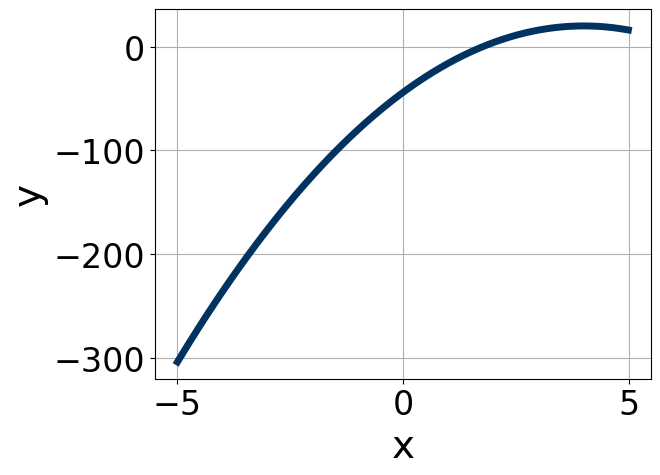
\includegraphics[width = 0.3\textwidth]{../Figures/quadraticEquationToGraphAB.png}\item 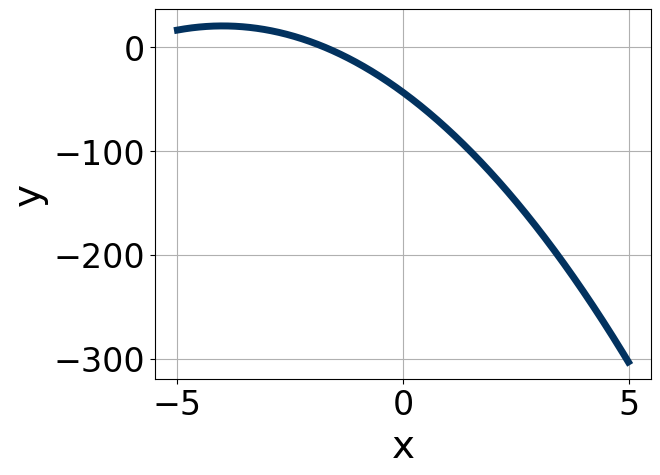
\includegraphics[width = 0.3\textwidth]{../Figures/quadraticEquationToGraphBB.png}\item 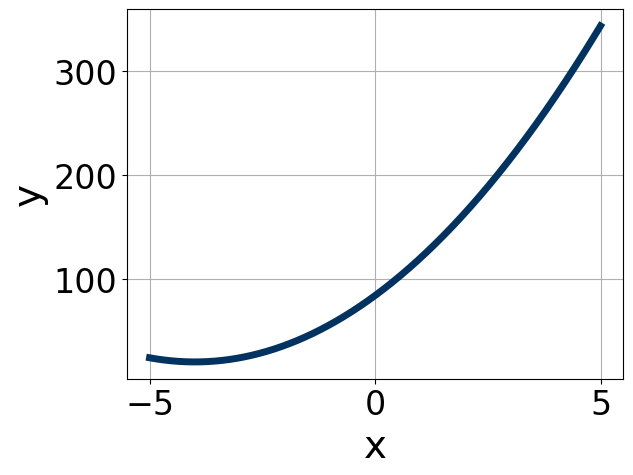
\includegraphics[width = 0.3\textwidth]{../Figures/quadraticEquationToGraphCB.png}\item 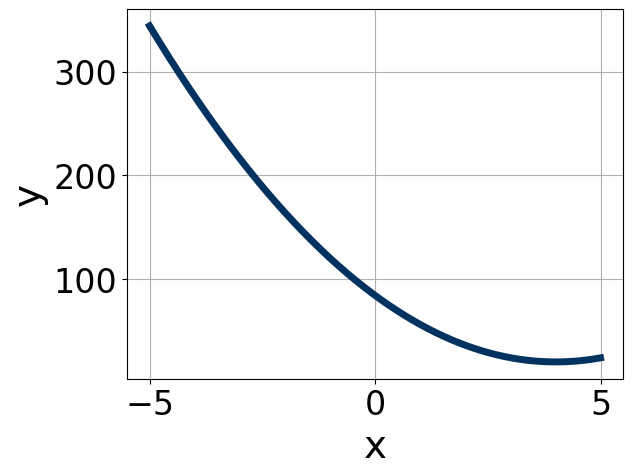
\includegraphics[width = 0.3\textwidth]{../Figures/quadraticEquationToGraphDB.png}\end{multicols}\item None of the above.
\end{enumerate} }
\litem{
Solve the quadratic equation below. Then, choose the intervals that the solutions $x_1$ and $x_2$ belong to, with $x_1 \leq x_2$.\[ 10x^{2} -57 x + 54 = 0 \]\begin{enumerate}[label=\Alph*.]
\item \( x_1 \in [-0.02, 0.46] \text{ and } x_2 \in [13.49, 13.9] \)
\item \( x_1 \in [11.96, 12.04] \text{ and } x_2 \in [44.69, 45.36] \)
\item \( x_1 \in [1.31, 1.77] \text{ and } x_2 \in [3.54, 4] \)
\item \( x_1 \in [1.07, 1.26] \text{ and } x_2 \in [4.47, 5.13] \)
\item \( x_1 \in [0.85, 1] \text{ and } x_2 \in [5.67, 7.13] \)

\end{enumerate} }
\litem{
Write the equation of the graph presented below in the form $f(x)=ax^2+bx+c$, assuming  $a=1$ or $a=-1$. Then, choose the intervals that $a, b,$ and $c$ belong to.
\begin{center}
    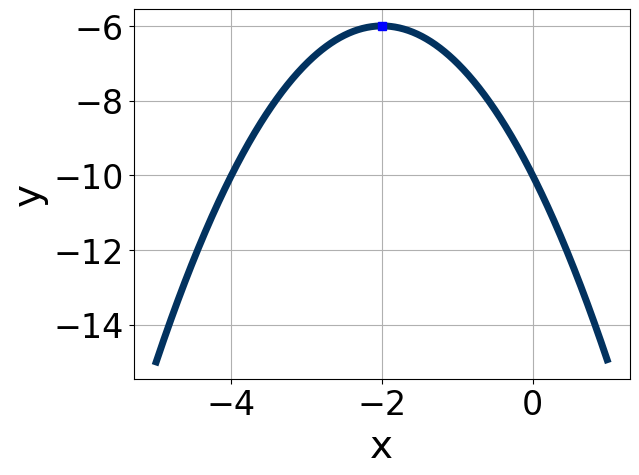
\includegraphics[width=0.5\textwidth]{../Figures/quadraticGraphToEquationB.png}
\end{center}
\begin{enumerate}[label=\Alph*.]
\item \( a \in [-1.8, 0.1], \hspace*{5mm} b \in [3, 8], \text{ and } \hspace*{5mm} c \in [-1, 4] \)
\item \( a \in [-1.8, 0.1], \hspace*{5mm} b \in [-5, -3], \text{ and } \hspace*{5mm} c \in [-13, -7] \)
\item \( a \in [-0.7, 1.6], \hspace*{5mm} b \in [3, 8], \text{ and } \hspace*{5mm} c \in [-3, 1] \)
\item \( a \in [-1.8, 0.1], \hspace*{5mm} b \in [3, 8], \text{ and } \hspace*{5mm} c \in [-13, -7] \)
\item \( a \in [-0.7, 1.6], \hspace*{5mm} b \in [-5, -3], \text{ and } \hspace*{5mm} c \in [-3, 1] \)

\end{enumerate} }
\litem{
Factor the quadratic below. Then, choose the intervals that contain the constants in the form $(ax+b)(cx+d); b \leq d.$\[ 54x^{2} +15 x -25 \]\begin{enumerate}[label=\Alph*.]
\item \( a \in [7.5, 11.6], \hspace*{5mm} b \in [-5, 2], \hspace*{5mm} c \in [6, 11], \text{ and } \hspace*{5mm} d \in [-1, 15] \)
\item \( a \in [2.6, 4.5], \hspace*{5mm} b \in [-5, 2], \hspace*{5mm} c \in [13, 20], \text{ and } \hspace*{5mm} d \in [-1, 15] \)
\item \( a \in [14.7, 19.6], \hspace*{5mm} b \in [-5, 2], \hspace*{5mm} c \in [3, 5], \text{ and } \hspace*{5mm} d \in [-1, 15] \)
\item \( a \in [-0.9, 1.2], \hspace*{5mm} b \in [-33, -27], \hspace*{5mm} c \in [0, 2], \text{ and } \hspace*{5mm} d \in [44, 52] \)
\item \( \text{None of the above.} \)

\end{enumerate} }
\litem{
Write the equation of the graph presented below in the form $f(x)=ax^2+bx+c$, assuming  $a=1$ or $a=-1$. Then, choose the intervals that $a, b,$ and $c$ belong to.
\begin{center}
    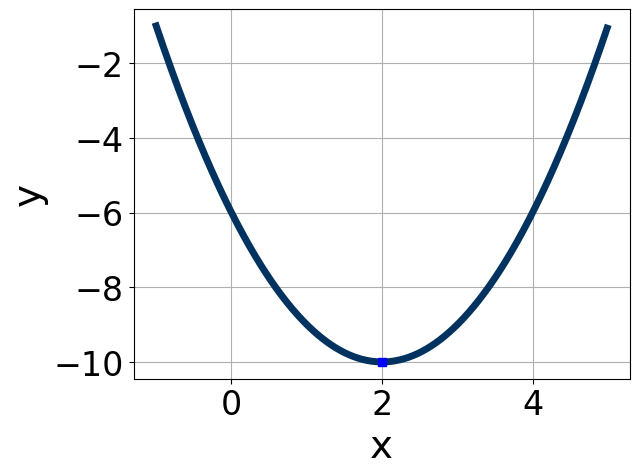
\includegraphics[width=0.5\textwidth]{../Figures/quadraticGraphToEquationCopyB.png}
\end{center}
\begin{enumerate}[label=\Alph*.]
\item \( a \in [-1, 0], \hspace*{5mm} b \in [-4, -2], \text{ and } \hspace*{5mm} c \in [-14, -11] \)
\item \( a \in [1, 3], \hspace*{5mm} b \in [4, 5], \text{ and } \hspace*{5mm} c \in [10, 16] \)
\item \( a \in [1, 3], \hspace*{5mm} b \in [-4, -2], \text{ and } \hspace*{5mm} c \in [-8, -5] \)
\item \( a \in [1, 3], \hspace*{5mm} b \in [4, 5], \text{ and } \hspace*{5mm} c \in [-8, -5] \)
\item \( a \in [-1, 0], \hspace*{5mm} b \in [4, 5], \text{ and } \hspace*{5mm} c \in [-14, -11] \)

\end{enumerate} }
\litem{
Graph the equation below.\[ f(x) = -(x-1)^2 + 11 \]\begin{enumerate}[label=\Alph*.]
\begin{multicols}{2}\item 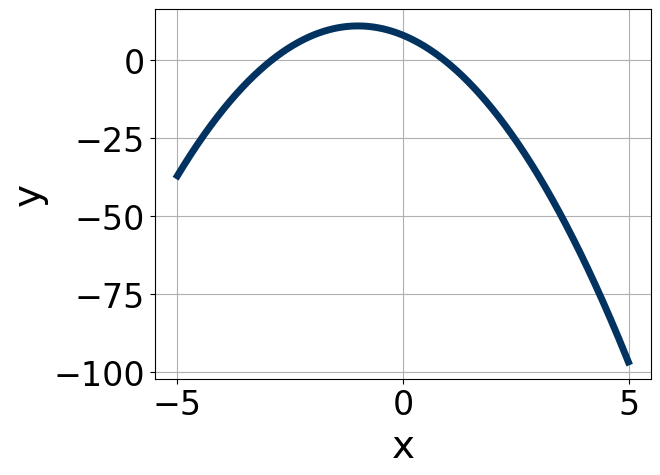
\includegraphics[width = 0.3\textwidth]{../Figures/quadraticEquationToGraphCopyAC.png}\item 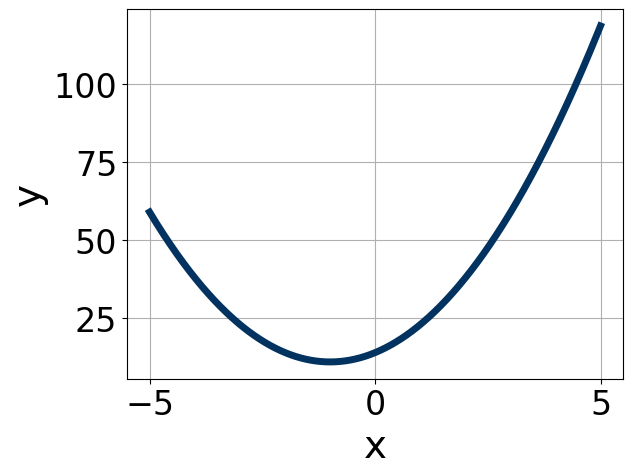
\includegraphics[width = 0.3\textwidth]{../Figures/quadraticEquationToGraphCopyBC.png}\item 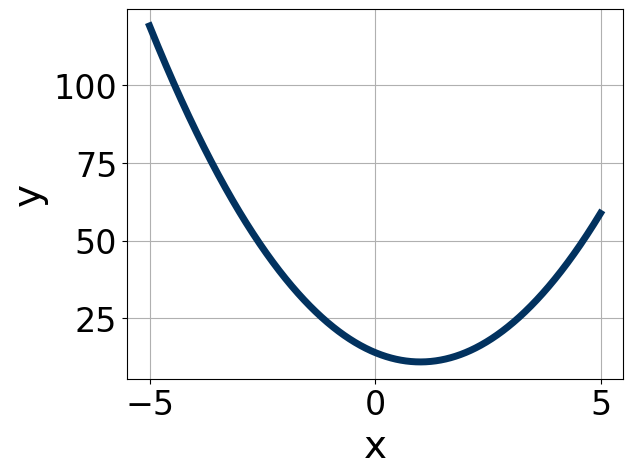
\includegraphics[width = 0.3\textwidth]{../Figures/quadraticEquationToGraphCopyCC.png}\item 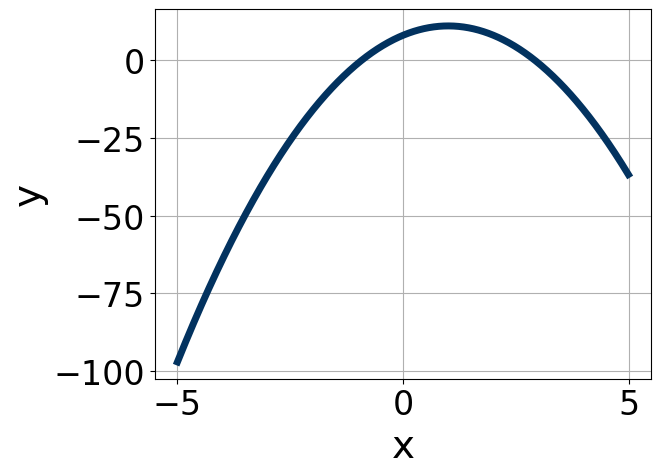
\includegraphics[width = 0.3\textwidth]{../Figures/quadraticEquationToGraphCopyDC.png}\end{multicols}\item None of the above.
\end{enumerate} }
\litem{
Solve the quadratic equation below. Then, choose the intervals that the solutions belong to, with $x_1 \leq x_2$ (if they exist).\[ 10x^{2} -13 x + 2 = 0 \]\begin{enumerate}[label=\Alph*.]
\item \( x_1 \in [-1.4, -0.1] \text{ and } x_2 \in [-0.18, 0.82] \)
\item \( x_1 \in [1.4, 2.4] \text{ and } x_2 \in [10.22, 12.22] \)
\item \( x_1 \in [-1.1, 1.2] \text{ and } x_2 \in [1.12, 6.12] \)
\item \( x_1 \in [-9, -8.5] \text{ and } x_2 \in [8.08, 11.08] \)
\item \( \text{There are no Real solutions.} \)

\end{enumerate} }
\litem{
Factor the quadratic below. Then, choose the intervals that contain the constants in the form $(ax+b)(cx+d); b \leq d.$\[ 81x^{2} +90 x + 25 \]\begin{enumerate}[label=\Alph*.]
\item \( a \in [-6, 2], \hspace*{5mm} b \in [41, 49], \hspace*{5mm} c \in [-0.4, 2.6], \text{ and } \hspace*{5mm} d \in [41, 52] \)
\item \( a \in [9, 10], \hspace*{5mm} b \in [5, 9], \hspace*{5mm} c \in [6.2, 12.3], \text{ and } \hspace*{5mm} d \in [0, 10] \)
\item \( a \in [22, 29], \hspace*{5mm} b \in [5, 9], \hspace*{5mm} c \in [1.7, 5], \text{ and } \hspace*{5mm} d \in [0, 10] \)
\item \( a \in [3, 7], \hspace*{5mm} b \in [5, 9], \hspace*{5mm} c \in [26.6, 27.5], \text{ and } \hspace*{5mm} d \in [0, 10] \)
\item \( \text{None of the above.} \)

\end{enumerate} }
\litem{
Solve the quadratic equation below. Then, choose the intervals that the solutions $x_1$ and $x_2$ belong to, with $x_1 \leq x_2$.\[ 25x^{2} +25 x -36 = 0 \]\begin{enumerate}[label=\Alph*.]
\item \( x_1 \in [-0.71, -0.32] \text{ and } x_2 \in [2.39, 2.41] \)
\item \( x_1 \in [-45.74, -44.28] \text{ and } x_2 \in [19.97, 20.18] \)
\item \( x_1 \in [-9.57, -7.92] \text{ and } x_2 \in [0.04, 0.25] \)
\item \( x_1 \in [-2.53, -1.43] \text{ and } x_2 \in [0.75, 0.81] \)
\item \( x_1 \in [-4.18, -3.5] \text{ and } x_2 \in [0.26, 0.64] \)

\end{enumerate} }
\litem{
Solve the quadratic equation below. Then, choose the intervals that the solutions belong to, with $x_1 \leq x_2$ (if they exist).\[ 11x^{2} -12 x + 3 = 0 \]\begin{enumerate}[label=\Alph*.]
\item \( x_1 \in [0.31, 0.51] \text{ and } x_2 \in [0.1, 0.8] \)
\item \( x_1 \in [3.88, 4.32] \text{ and } x_2 \in [6.8, 8] \)
\item \( x_1 \in [-3.3, -2.62] \text{ and } x_2 \in [2.1, 4.3] \)
\item \( x_1 \in [-1.63, 0.2] \text{ and } x_2 \in [-0.9, 0.2] \)
\item \( \text{There are no Real solutions.} \)

\end{enumerate} }
\litem{
Graph the equation below.\[ f(x) = -(x+1)^2 + 20 \]\begin{enumerate}[label=\Alph*.]
\begin{multicols}{2}\item 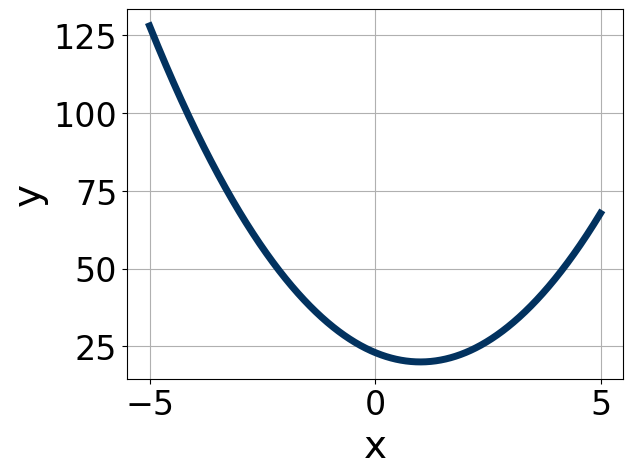
\includegraphics[width = 0.3\textwidth]{../Figures/quadraticEquationToGraphAC.png}\item 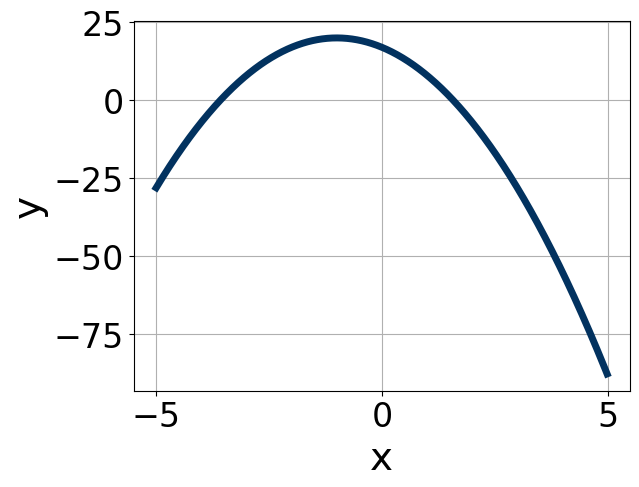
\includegraphics[width = 0.3\textwidth]{../Figures/quadraticEquationToGraphBC.png}\item 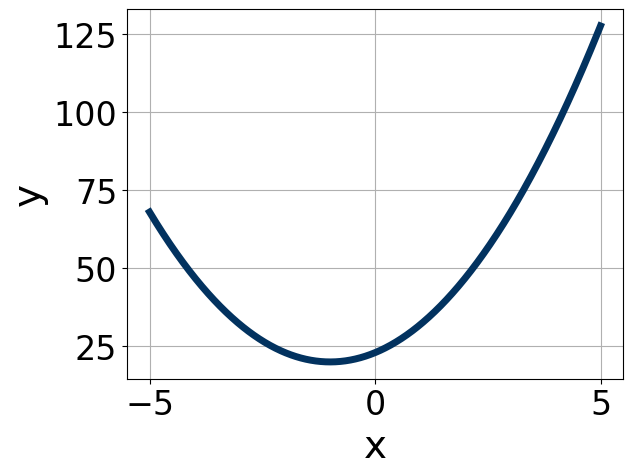
\includegraphics[width = 0.3\textwidth]{../Figures/quadraticEquationToGraphCC.png}\item 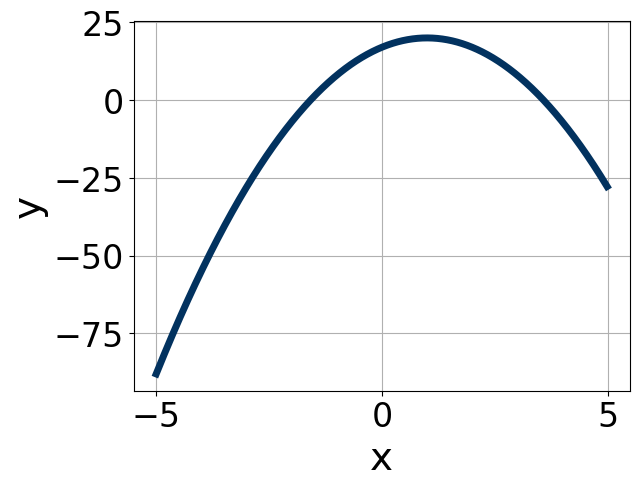
\includegraphics[width = 0.3\textwidth]{../Figures/quadraticEquationToGraphDC.png}\end{multicols}\item None of the above.
\end{enumerate} }
\litem{
Solve the quadratic equation below. Then, choose the intervals that the solutions $x_1$ and $x_2$ belong to, with $x_1 \leq x_2$.\[ 25x^{2} -50 x + 24 = 0 \]\begin{enumerate}[label=\Alph*.]
\item \( x_1 \in [0.18, 0.28] \text{ and } x_2 \in [3.53, 4.07] \)
\item \( x_1 \in [0.62, 0.83] \text{ and } x_2 \in [0.84, 1.28] \)
\item \( x_1 \in [19.98, 20.03] \text{ and } x_2 \in [29.73, 30.11] \)
\item \( x_1 \in [0.55, 0.73] \text{ and } x_2 \in [1.47, 2.23] \)
\item \( x_1 \in [0.33, 0.55] \text{ and } x_2 \in [1.9, 2.69] \)

\end{enumerate} }
\litem{
Write the equation of the graph presented below in the form $f(x)=ax^2+bx+c$, assuming  $a=1$ or $a=-1$. Then, choose the intervals that $a, b,$ and $c$ belong to.
\begin{center}
    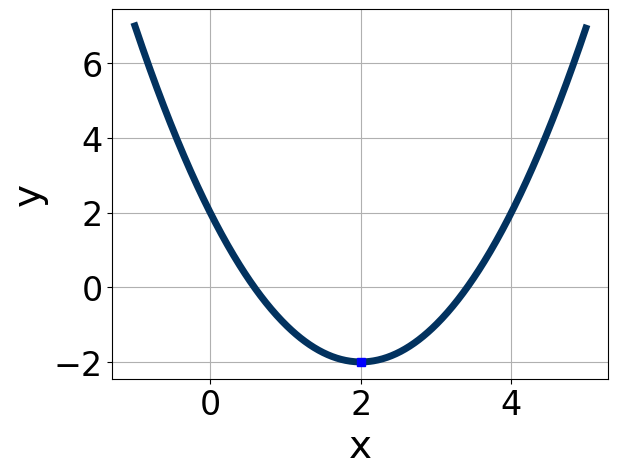
\includegraphics[width=0.5\textwidth]{../Figures/quadraticGraphToEquationC.png}
\end{center}
\begin{enumerate}[label=\Alph*.]
\item \( a \in [-1, 0], \hspace*{5mm} b \in [4, 7], \text{ and } \hspace*{5mm} c \in [-7, -4] \)
\item \( a \in [0, 5], \hspace*{5mm} b \in [4, 7], \text{ and } \hspace*{5mm} c \in [0, 4] \)
\item \( a \in [0, 5], \hspace*{5mm} b \in [4, 7], \text{ and } \hspace*{5mm} c \in [4, 8] \)
\item \( a \in [0, 5], \hspace*{5mm} b \in [-4, -3], \text{ and } \hspace*{5mm} c \in [0, 4] \)
\item \( a \in [-1, 0], \hspace*{5mm} b \in [-4, -3], \text{ and } \hspace*{5mm} c \in [-7, -4] \)

\end{enumerate} }
\litem{
Factor the quadratic below. Then, choose the intervals that contain the constants in the form $(ax+b)(cx+d); b \leq d.$\[ 54x^{2} -69 x + 20 \]\begin{enumerate}[label=\Alph*.]
\item \( a \in [5.94, 7.72], \hspace*{5mm} b \in [-5, -3], \hspace*{5mm} c \in [5, 13], \text{ and } \hspace*{5mm} d \in [-6, -3] \)
\item \( a \in [0.23, 1.4], \hspace*{5mm} b \in [-49, -43], \hspace*{5mm} c \in [1, 3], \text{ and } \hspace*{5mm} d \in [-24, -23] \)
\item \( a \in [1.09, 2.11], \hspace*{5mm} b \in [-5, -3], \hspace*{5mm} c \in [27, 28], \text{ and } \hspace*{5mm} d \in [-6, -3] \)
\item \( a \in [11.78, 12.62], \hspace*{5mm} b \in [-5, -3], \hspace*{5mm} c \in [3, 6], \text{ and } \hspace*{5mm} d \in [-6, -3] \)
\item \( \text{None of the above.} \)

\end{enumerate} }
\litem{
Write the equation of the graph presented below in the form $f(x)=ax^2+bx+c$, assuming  $a=1$ or $a=-1$. Then, choose the intervals that $a, b,$ and $c$ belong to.
\begin{center}
    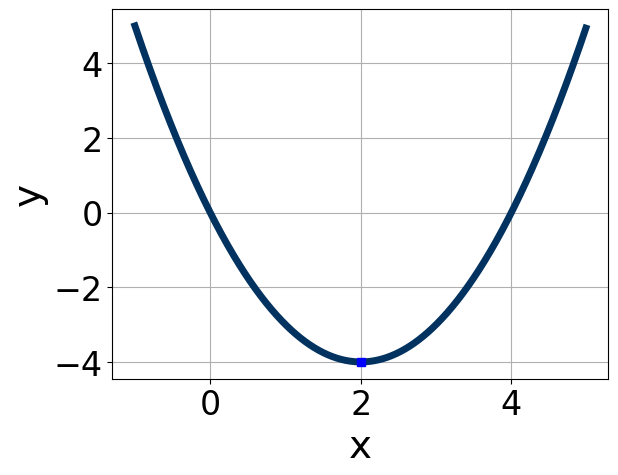
\includegraphics[width=0.5\textwidth]{../Figures/quadraticGraphToEquationCopyC.png}
\end{center}
\begin{enumerate}[label=\Alph*.]
\item \( a \in [0.5, 2.3], \hspace*{5mm} b \in [2, 6], \text{ and } \hspace*{5mm} c \in [-1, 1] \)
\item \( a \in [-1.2, 0.5], \hspace*{5mm} b \in [2, 6], \text{ and } \hspace*{5mm} c \in [-8, -5] \)
\item \( a \in [-1.2, 0.5], \hspace*{5mm} b \in [-7, 0], \text{ and } \hspace*{5mm} c \in [-8, -5] \)
\item \( a \in [0.5, 2.3], \hspace*{5mm} b \in [-7, 0], \text{ and } \hspace*{5mm} c \in [-1, 1] \)
\item \( a \in [0.5, 2.3], \hspace*{5mm} b \in [2, 6], \text{ and } \hspace*{5mm} c \in [8, 10] \)

\end{enumerate} }
\end{enumerate}

\end{document}